\documentclass[journal]{vgtc}                % final (journal style)
%\documentclass[review,journal]{vgtc}         % review (journal style)
%\documentclass[widereview]{vgtc}             % wide-spaced review
%\documentclass[preprint,journal]{vgtc}       % preprint (journal style)

%% Uncomment one of the lines above depending on where your paper is
%% in the conference process. ``review'' and ``widereview'' are for review
%% submission, ``preprint'' is for pre-publication, and the final version
%% doesn't use a specific qualifier.

%% Please use one of the ``review'' options in combination with the
%% assigned online id (see below) ONLY if your paper uses a double blind
%% review process. Some conferences, like IEEE Vis and InfoVis, have NOT
%% in the past.

%% Please note that the use of figures other than the optional teaser is not permitted on the first page
%% of the journal version.  Figures should begin on the second page and be
%% in CMYK or Grey scale format, otherwise, colour shifting may occur
%% during the printing process.  Papers submitted with figures other than the optional teaser on the
%% first page will be refused. Also, the teaser figure should only have the
%% width of the abstract as the template enforces it.

%% These few lines make a distinction between latex and pdflatex calls and they
%% bring in essential packages for graphics and font handling.
%% Note that due to the \DeclareGraphicsExtensions{} call it is no longer necessary
%% to provide the the path and extension of a graphics file:
%% 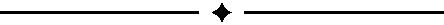
\includegraphics{diamondrule} is completely sufficient.
%%
\ifpdf%                                % if we use pdflatex
  \pdfoutput=1\relax                   % create PDFs from pdfLaTeX
  \pdfcompresslevel=9                  % PDF Compression
  \pdfoptionpdfminorversion=7         % create PDF 1.7
  \ExecuteOptions{pdftex}
  \usepackage{graphicx}  
  \graphicspath{ {pictures/} }              % allow us to embed graphics files
  \DeclareGraphicsExtensions{.pdf,.png,.jpg,.jpeg} % for pdflatex we expect .pdf, .png, or .jpg files
\else%                                 % else we use pure latex
  \ExecuteOptions{dvips}
  \usepackage{graphicx}                % allow us to embed graphics files
  \DeclareGraphicsExtensions{.eps}     % for pure latex we expect eps files
\fi%

%% it is recomended to use ``\autoref{sec:bla}'' instead of ``Fig.~\ref{sec:bla}''
\graphicspath{{figures/}{pictures/}{images/}{./}} % where to search for the images

\usepackage{microtype}                 % use micro-typography (slightly more compact, better to read)
\PassOptionsToPackage{warn}{textcomp}  % to address font issues with \textrightarrow
\usepackage{textcomp}                  % use better special symbols
\usepackage{mathptmx}                  % use matching math font
\usepackage{times}                     % we use Times as the main font
\renewcommand*\ttdefault{txtt}         % a nicer typewriter font
\usepackage{cite}                      % needed to automatically sort the references
\usepackage{tabu}                      % only used for the table example
\usepackage{booktabs}                  % only used for the table example
\usepackage[section]{placeins}
\usepackage{float}
\usepackage{hyperref}
\usepackage[all]{hypcap}
\usepackage{enumitem}
\usepackage[hyphenbreaks]{breakurl}
\hypersetup{
    colorlinks = true,
    citecolor = {green},
    urlcolor = {red}
}
%% We encourage the use of mathptmx for consistent usage of times font
%% throughout the proceedings. However, if you encounter conflicts
%% with other math-related packages, you may want to disable it.

%% In preprint mode you may define your own headline.
%\preprinttext{To appear in IEEE Transactions on Visualization and Computer Graphics.}

%% If you are submitting a paper to a conference for review with a double
%% blind reviewing process, please replace the value ``0'' below with your
%% OnlineID. Otherwise, you may safely leave it at ``0''.
\onlineid{0}

%% declare the category of your paper, only shown in review mode
\vgtccategory{Research}
%% please declare the paper type of your paper to help reviewers, only shown in review mode
%% choices:
%% * algorithm/technique
%% * application/design study
%% * evaluation
%% * system
%% * theory/model

%% Paper title.
\title{Crimes on Oregon College Campuses}

%% This is how authors are specified in the journal style

%% indicate IEEE Member or Student Member in form indicated below
\author{Daniel Schroeder, Joseph Boyd, and Siva Pranav Kumar Timmireddy}
\authorfooter{
%% insert punctuation at end of each item
\item
 Daniel Schroeder is a computer science student at Oregon State University. E-mail: schrodan@oregonstate.edu.
\item
 Joseph Boyd is a mechanical engineering Masters student at Oregon State University. Email: boydjo@oregonstate.edu.
\item
 Siva Pranav Kumar Timmireddy is an electronics and computer engineering Master student at Oregon State University. E-mail: timmires@oregonstate.edu.
}

%other entries to be set up for journal
%\shortauthortitle{Biv \MakeLowercase{\textit{et al.}}: Crimes on Oregon College Campuses}
%\shortauthortitle{Firstauthor \MakeLowercase{\textit{et al.}}: Paper Title}

%% Abstract section.
\abstract{This paper is an explanation of our data visualization webpage for crimes on college campuses. We gathered a public federal database of reported crimes on college campuses across the United States and attempted to create a visualization to easily represent the data. This paper presents the questions, issues, research, and implementation of our visualization along with the reasoning for the decisions made throughout the process. %
} % end of abstract

%% Keywords that describe your work. Will show as 'Index Terms' in journal
%% please capitalize first letter and insert punctuation after last keyword
\keywords{Data Visualization, Campus Crimes, Oregon State University, Portland State University,
University of Oregon, Bar Graph}

%% ACM Computing Classification System (CCS). 
%% See <http://www.acm.org/class/1998/> for details.
%% The ``\CCScat'' command takes four arguments.

\CCScatlist{ % not used in journal version
 \CCScat{K.6.1}{Management of Computing and Information Systems}%
{Project and People Management}{Life Cycle};
 \CCScat{K.7.m}{The Computing Profession}{Miscellaneous}{Ethics}
}

%% Uncomment below to include a teaser figure.
\teaser{
  \centering
  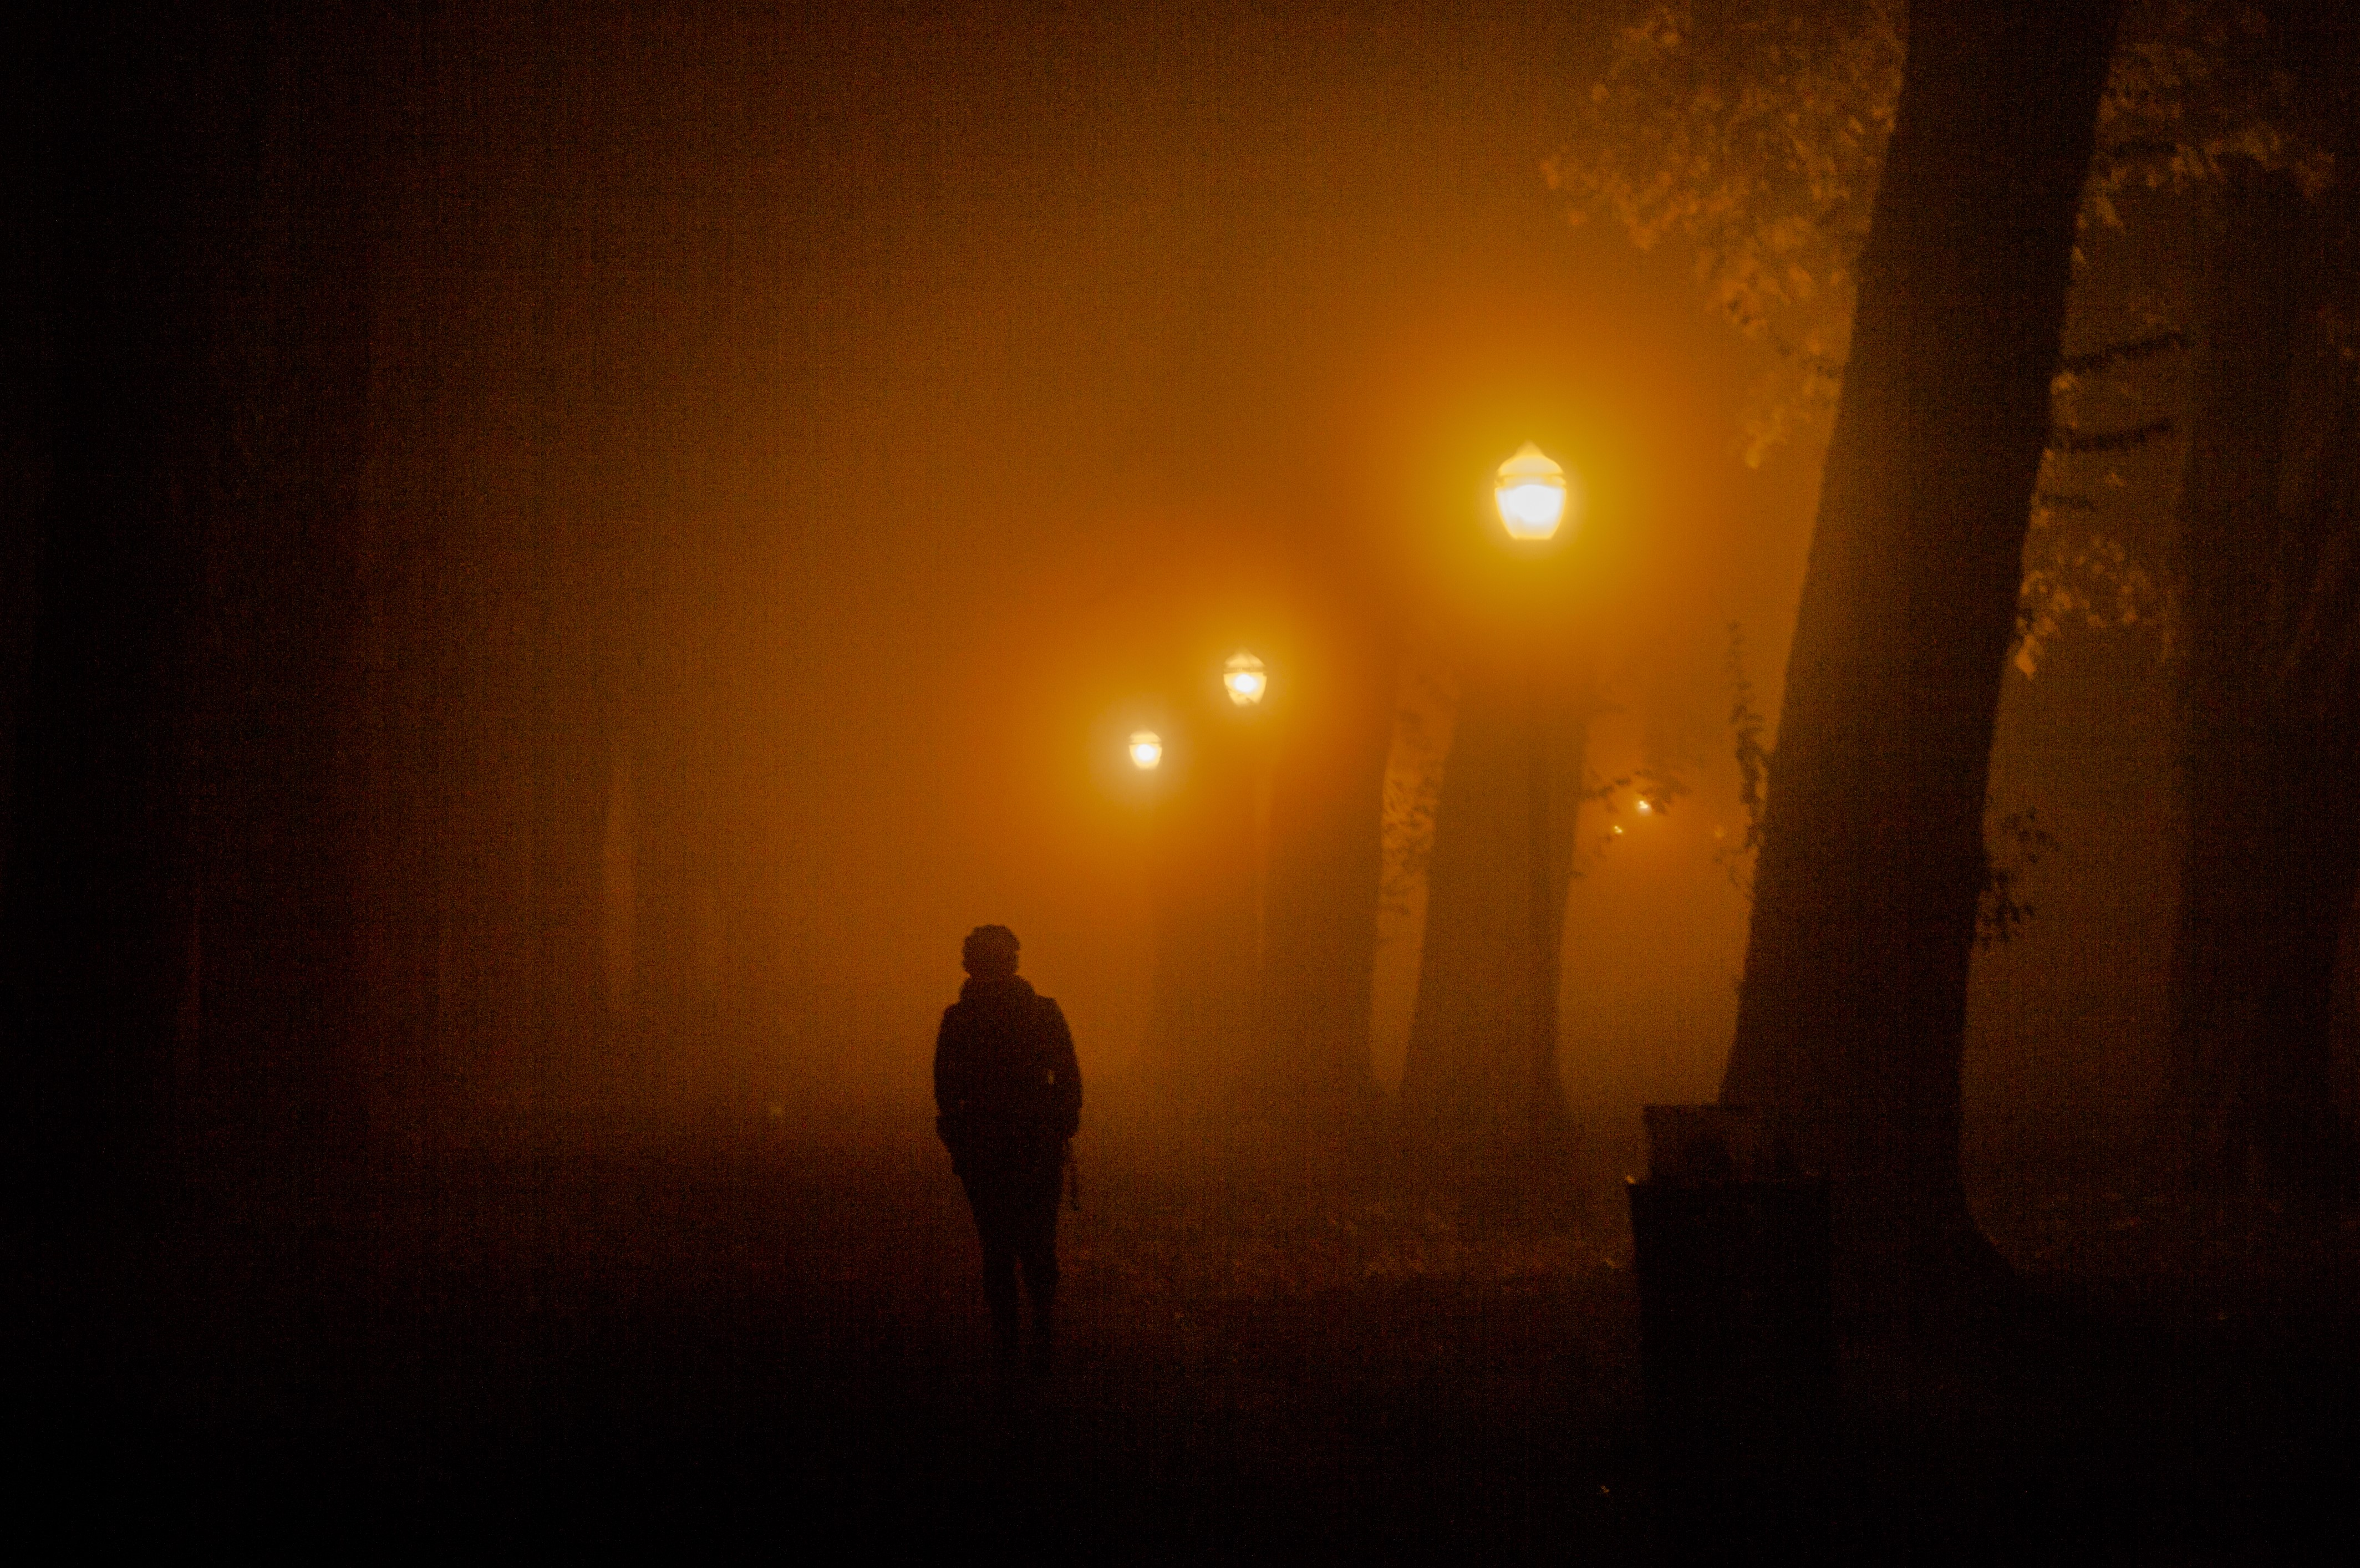
\includegraphics[width=\linewidth, height=3.5in]{FF}
  \caption{Photo by: Zach Freedel. The photo of the fog was taken in Corvallis, Oregon, on the campus of Oregon State University.}
	\label{fig:teaser}
}

%% Uncomment below to disable the manuscript note
\renewcommand{\manuscriptnotetxt}{}

%% Copyright space is enabled by default as required by guidelines.
%% It is disabled by the 'review' option or via the following command:
% \nocopyrightspace

\vgtcinsertpkg

%%%%%%%%%%%%%%%%%%%%%%%%%%%%%%%%%%%%%%%%%%%%%%%%%%%%%%%%%%%%%%%%
%%%%%%%%%%%%%%%%%%%%%% START OF THE PAPER %%%%%%%%%%%%%%%%%%%%%%
%%%%%%%%%%%%%%%%%%%%%%%%%%%%%%%%%%%%%%%%%%%%%%%%%%%%%%%%%%%%%%%%%

\begin{document}

%% The ``\maketitle'' command must be the first command after the
%% ``\begin{document}'' command. It prepares and prints the title block.

%% the only exception to this rule is the \firstsection command
\firstsection{Introduction}

\maketitle

The safety of students at a university is of utmost importance. The crime rate in and around the university plays a vital role when students begin to choose their desired schools. With this project, we intend to help young students and parents make well-informed decisions when searching for potential colleges as well as help universities to improve security. The Department of Education released this data set which contains the information of campus arrests and crimes in the years 2013, 2014, 2015.\\
\indent Our webpage visualization allows the users to compare universities based on reported campus arrests. However, currently there is no known visualization that portrays this data, let alone in a fashionable and user-friendly manner. The problem that this paper addresses is how this dataset can be visualized to provide valuable insight for students seeking information about university safety. The Department of Education dataset has approximately 11,300 rows of data pertaining to the locations of university campus arrests. There are sometimes multiple rows for one university; a row for arrests made on the main campus, a row for arrests made in on-campus housing, etc. This presented some difficulty in gathering the correct data for each university through which we overcame by merging rows with mutual institution name columns and creating a collection of all the data for a specific university.\\
\indent The aim of this visualization is to map recorded crimes committed on Oregon State University, University of Oregon, and Portland State University campuses onto a map of Oregon, and then show the different crimes committed in the form bar charts. As the dataset is huge and handling such a vast dataset may result in complications while visualizing, we have decided to first start with the selected Oregon universities and eventually include all the universities and colleges across the United States. The visualization is a good way to represent this data set as it makes it easier for the intended audience to understand the data through graphical representation and a visually appealing interface.\\ \\
\newline
\newline
\newline
The work presented here yields the following benefits and contributions:
\begin{itemize}
\setlength\itemsep{0em}
\item Our visualization provides a way to easily visualize college crimes that has not been previously implemented.
\item We use filters that allow comparisons within a single university (\autoref{fig:OneSchoolAllData}) and comparisons between multiple universities (\autoref{fig:AllSchoolsOneType}).
\item Our visualization can be easily reconstructed to satisfy any collection of universities and crimes.
\end{itemize}
\indent The following paper is organized into the following sections.  Section 2 (\nameref{research}) introduces the research done in order to properly plan and implement our visualization. Section 3 (\nameref{methods}) explains the methods of implementation and how the desired webpage was constructed. Lastly, Section 4 (\nameref{conclusion}) introduces a conclusive summary with insight on future plans of improvement and how effective our visualization was in addressing our issue.\\

\section{Literary Research and References} \label{research}
The data for crimes committed on campuses in the United States has been required by the Clery Act law to be sent to the government each year.  However, this raw data is of little help to future students and parents, because it is presented as long reports of numbers that are hard to gather any information from\cite{lipka-2011}.  A web based visualization will enable future students to easily find the crime data without sorting through dense reports.

A study in 2012 showed that students were afraid of crime maps as it made crimes seem more prevalent than they actually were\cite{fuhrmann-huynh-scholz-2013}. In their visualization they used a bivariate mapping technique to show the actual reported crimes versus the student’s fear of crimes.  For our visualization, we compare reported crimes based on crime type and school, so a different approach is needed.  The same base numbers are used for each University so each of them can be easily compared to one another.  The only downside to this method is that the size of the University is not taken into account which may make smaller Universities disproportionately more safe.

The data accessible to us is on-campus only. The problem with this is that locations not on campus can contribute to crime stats without being explicitly school related.  A report shows the Casinos near campus can cause spikes in certain crimes.  Robberies and vehicle thefts near the college campus increased, but burglaries are lower\cite{Thomas:2011:CRIME}.  However, for our project, this does not change the base crime statistics.
Other problems with our visualization is that it only shows successful crimes that are reported.  Universities have several methods in place to alleviate crime and make their campuses safer\cite{doi:10.1177/0193841X13509815}.  Emergency phones and well lit walkways are just some of the infrastructure in place to counter crime.  In our data, only the resulting crime is reported.

One visualization for crime statistics is shown on funcvis.org\cite{kogan_2013}.  This method was to show a ``bubble plot'' to visualize the crime statistics per population.  We liked the functionality for dynamically changing the visual based on the filters chosen.  This enabled the viewer to focus on what crimes they were most concerned/interested in.  However, a couple of problems were with this approach.  Firstly, it presented information as a proportion of all elements rather than an explicit representation of the data values would show in a bar graph.  Secondly, the ``bubbles'' had to be searched if the viewer wanted to know a specific state.  To solve these problems, we used a geospatial interface based on the university and a bar graph.\\
A visualization similar to ours was completed in 2015 for a project\cite{holloway-2015}.  This visualization also used the bubble plot type using sizes for number of crimes.  The user can zoom into the visualization to show the divide between public and private universities (2 and 4 years).  While this is useful in showing the relative amount of crimes committed it does not show the base numbers, where our visualization use the base numbers to give the user more information.  In addition, our visualization allows search by college, something unable to be done by the other visualization.\\
Finally, an extensive visualization project was published to the web from the University of Maryland, College Park\cite{cho-liu-2009}.  This visualization uses data from UM to compare crimes using Spotfire and Timesearcher.  While extensive, Spotfire uses a treemap visualization method to show the amount of crimes committed per location.  While this helps show what area is the most crime affected, the tree method makes it hard to find a specific location since the are too small to see.  The use of Timesearcher, a simple dot and line graph, to show the times during what crimes are committed is useful but it is also too hard to read as it is all in monochrome.\\
\section{Method and Implementation} \label{methods}

For this visualization, we created a webpage \href{http://people.oregonstate.edu/~schrodan/}{Crimes on Oregon College Campuses} (\href{http://people.oregonstate.edu/~schrodan/}{http://people.oregonstate.edu/~schrodan/}) that implements the d3.js v4 package to gather data and present a graphic representation. We had a public dataset \href{https://ope.ed.gov/campussafety/#/}{Campus Crimes and Safety} with campus crime data from 2013, 2014, and 2015 for colleges all over the united states. From that data, we selected rows pertaining to Oregon colleges (specifically Oregon State University, University of Oregon, and Portland State University) and loaded them as a .csv file into the d3 JavaScript of our webpage. Our visualization creates a dynamic bar chart that changes according to the different filters applied.\\
\indent Our group researched several different visualization techniques in the previous section (\nameref{research}) including pie charts, bubble maps, and heap maps that were used to display data. We analyzed the reasoning behind each technique and began to consider what we really want to convey with our visualization. Some visualizations aimed to display proportionalities between geographical areas or data categories. Some visualizations wanted to show concentrations of data for specific regions with heap maps. For our design, we chose to use bar charts for our visualization so that users can clearly depict the values for each bar through the use of axes labels and ticks.\\
\indent Our visualization presents college campus crime data through three main comparisons:
\begin{enumerate}
	\setlength\itemsep{0em}
	\item Liquor, weapon, and drug crimes for the years 2013-2015 for a given university.
	\item A comparison of each crime type per each year (i.e. weapons crimes of 2013, 2014, and 2015).
	\item A comparison of all school's crimes for a given crime type (All Oregon State weapon crimes vs. all University of Oregon weapon crimes vs. all Portland State weapon crimes).
\end{enumerate}

\begin{figure}[H]
\label{fig:OverviewDiagram}
\centering
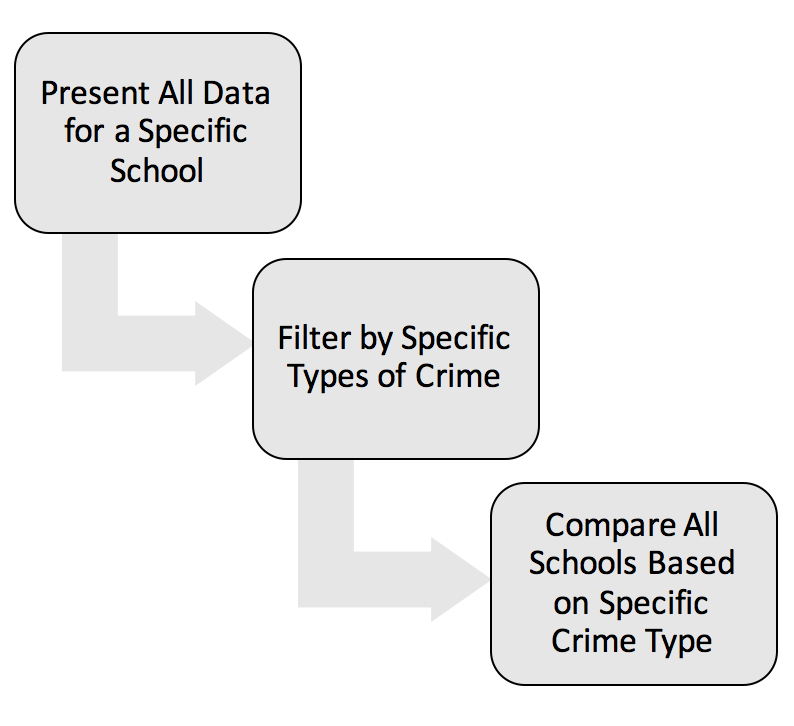
\includegraphics[width=6cm, height=6cm]{method-flow-chart}
\caption{Overview Diagram of Visualization Model}
\end{figure}
We use a simple button group that dynamically changes the d3 svg object according to the desired filter. We accomplish this by updating the dataset given to the d3 axes and bar objects each time a new filter event is activated. 
\subsection{One School, All Data}
Our visualization begins by selecting a school from an image of the state of Oregon and displaying crime data for weapon crimes, drug crimes, and liquor crimes by year. By clicking on a school node, the webpage calls a JavaScript function buildChart() and passes in a string parameter for the desired college. This function then parses the .csv file and creates arrays for each crime type and year based on college. We used d3.js functions such as nest() and rollup() to combine all data rows for the same college and add the values for each crime category \cite{d3API}.
It then creates a dataset by selecting only data from each array pertaining to the college supplied by the function parameter. Using this dataset, the function appends rectangle objects and axes to the svg element in the HTML of the webpage, and populates each obbject with the corresponding values. This creates a bar graph separated by crime type and year for the specified school. Clicking a different college node on the map image will remove all previous rectangles and axes, repopulate the dataset with the corresponding college's data, and rebuild the bar graph. 
\begin{figure}[H]
\label{fig:OneSchoolAllData} 
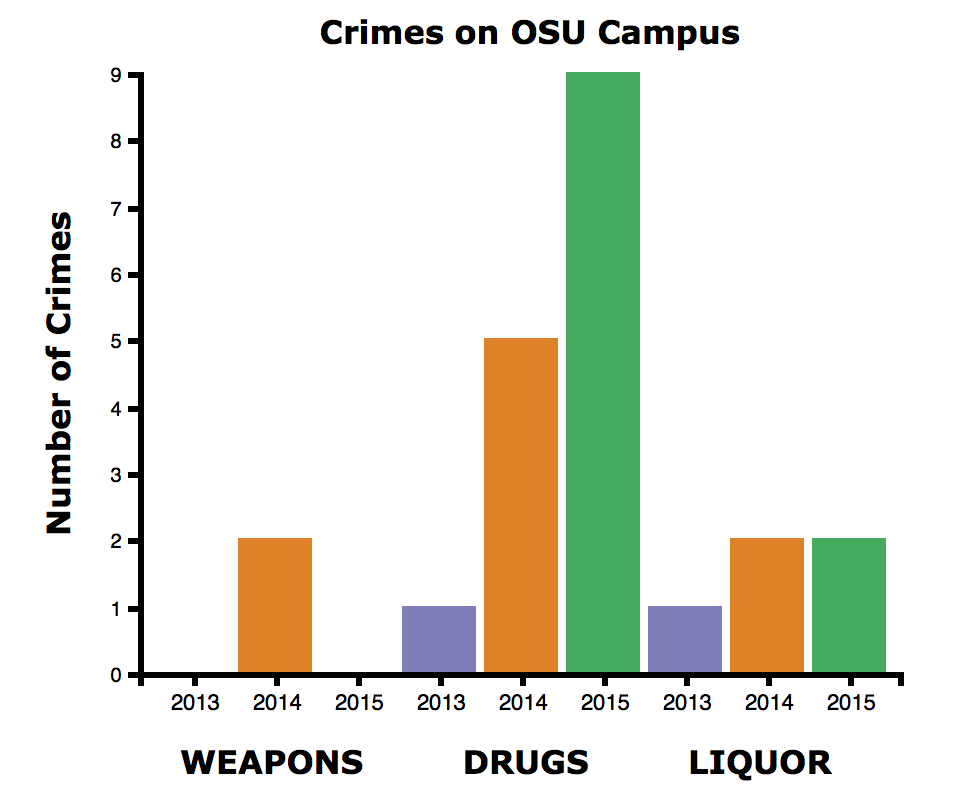
\includegraphics[width=8cm, height=7cm]{OneSchoolAllData}
\caption{A bar graph of all crimes for Oregon State University organized by crime type and year.}
\end{figure}

\subsection{One School, By Crime Type}
Our visualization adopts filtering techniques made aware to us by one of our researched sources \cite{ kogan_2013 }, that allows the user to select a specific type of crime and see the number of reports of that crime by year.  This filter enables an explicit representation of crimes over time to depict whether a college campus has grown safer, or more dangerous, across the three years our dataset provided. There are HTML buttons pertaining to each type of crime (weapon, drug, and liquor), and upon clicking a button, one of three JavaScript functions pertaining to a crime type removes all d3 axes and rectangle objects from the current svg and updates the dataset by selecting the .cvs columns that correlate to the specified crime type. The function looks at what college is currently being displayed and builds a new bar chart with the specified crime type values for each year. As shown in \autoref{fig:OneSchoolOneType}, this bar graph shows an increase in drug crimes on Oregon State University's campus from 2013 to 2015 and provides a very clear, distinguishable comparison between each year.
\begin{figure}[H]
\label{fig:OneSchoolOneType} 
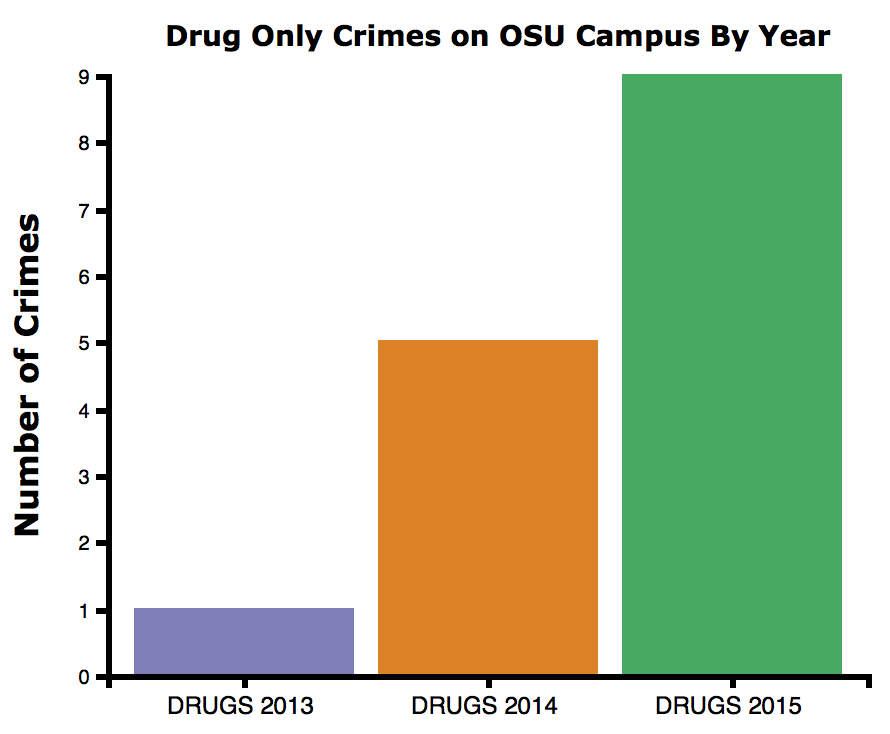
\includegraphics[width=8cm, height=7cm]{OneSchoolOneType}
\caption{A bar graph of all drug crimes for Oregon State University organized by year.}
\end{figure}

\subsection{All Schools, By Crime Type}
Our final component in the visualization compares all three colleges based on a given crime type. This filter provides a specific comparison between multiple college campuses rather than comparisons of crime data for one campus over time. We implemented this filter to provide users with the capability of visualizing data for multiple colleges side-by-side and being able to compare their values. This is similar to the idea of the ``bubble map’’ from \href{http://funcvis.org/visuals/crime/#all_states=&crimes=}{Crime Bubble Map} that allows different states to be compared visually by size of bubble, except, as previously stated, we wanted to visualized hard number values to the given representation. For this reason, we made each college its own bar in the graph so that the y-axis can properly represent the number values.
\begin{figure}[H]
\label{fig:AllSchoolsOneType}

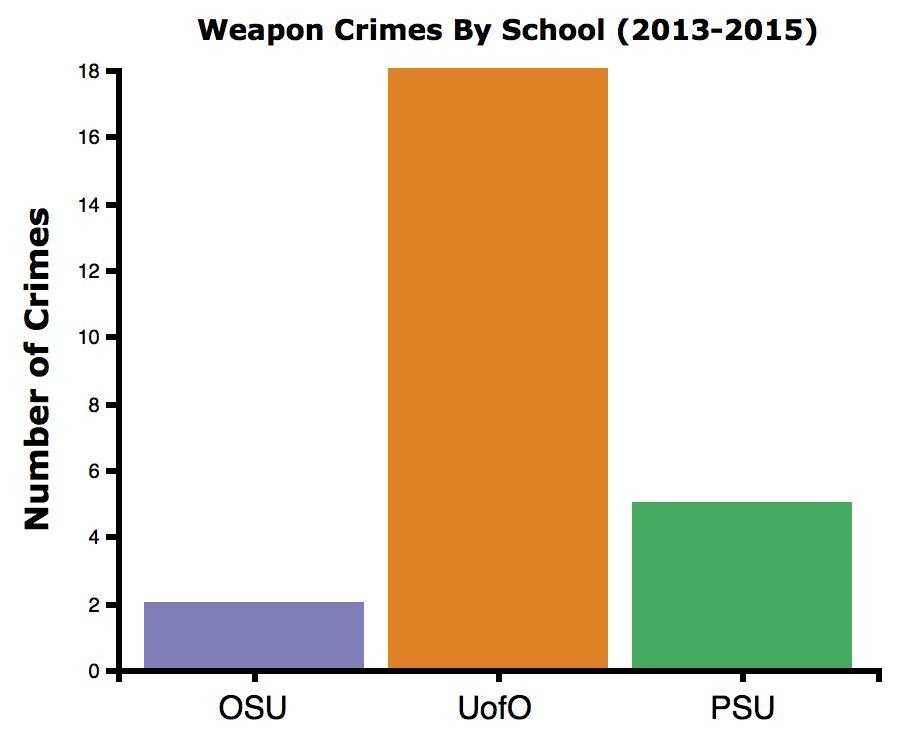
\includegraphics[width=8cm, height=7cm]{AllSchoolsOneType}
\caption{A bar graph of all weapon crimes for all three colleges from 2013 to 2015.}
\end{figure}

Each bar chart utilizes labels and axes to help explain the data presented. We chose three colors from the rgb range that were easily distinguishable when presented side-by-side. We could have used any red-based, blue-based, and green-based colors we wanted, but we found the colors displayed above to be aesthetically pleasing. They are soft colors that do not alarm the user when presented. This is beneficial when the user applies filters to create new charts, so that when displayed, the graphs are easy to the eye and seem appropriate. We also chose to use the same green that is in the bar charts for the header space and button group background colors. We chose this particular green so that it would match the graphs and not over-complicate the web page as well as to compliment the general theme of Oregon. These colors can be easily changed in the JavaScript of the webpage to better suit future projects that may not pertain to the state of Oregon or that may wish to use a different color scheme.


\section{Conclusion} \label{conclusion}

The problem of visualizing a dataset with different categories can be solved by deciding how to manage the data depending on the functionality and audience of the visualization. Our visualization mainly focuses on providing students and parents with an easy-to-use tool to make well informed decisions. We also try to provide universities with a capable tool to help compare their crime rate statistics to other schools.
This visualization achieves both the goals. The feature that allows comparisons of all the schools in one visual is meant mainly for students. Tracking the changes of different crimes over the years helps the universities understand the factors behind the patterns observed.
The visualization can be further improved by expanding it to the whole country, and including all the colleges. However, by doing so we populate the map with almost 11,000 nodes or schools. Having filters and allowing the users to select schools by geographic location or conference could be a future modification. The problem with disproportionate enrollment between schools can be solved by using the number of crimes per 1000 students. The dataset could also be used to make a heat map for each year and each category of crime which allows the users to analyze the data clearly and easily on a wider scale. 
%% if specified like this the section will be committed in review mode
\acknowledgments{
The authors wish to thank The Department of Education for the data provided as well as professor Eugene Zhang and teaching assistant Islam Al Musaly.}

%\bibliographystyle{abbrv}
\bibliographystyle{abbrv-doi}
%\bibliographystyle{abbrv-doi-narrow}
%\bibliographystyle{abbrv-doi-hyperref}
%\bibliographystyle{abbrv-doi-hyperref-narrow}

\bibliography{crimeoncampus}
\end{document}

